\documentclass{standalone}
\usepackage{tikz}
\usetikzlibrary{automata,positioning}

\begin{document}
  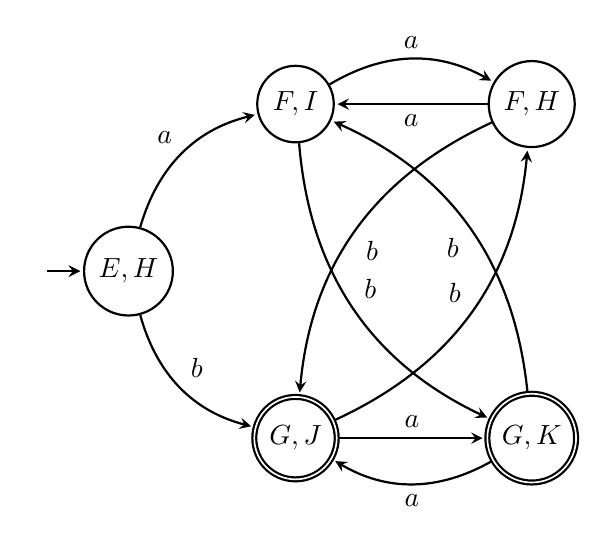
\begin{tikzpicture}[%
    >=stealth,
    shorten >=1pt,
    node distance=3cm,
    on grid,
    auto,
    state/.append style={minimum size=2em},
    thick
  ]
    \node[state, initial, initial text = {}] (A) {$E, H$};
    \node[state] (B) [above right of=A] {$F, I$};
    \node[state] (C) [accepting, below right of=A] {$G, J$};
    \node[state] (D) [right of=B] {$F, H$};
    \node[state] (E) [accepting, right of=C] {$G, K$};

    \path[->] (A) +(-1,0) edge (A)
              (A)         edge [bend left]  node {$a$} (B)
              (A)         edge [bend right] node {$b$} (C)
              (B)         edge [bend left]  node {$a$} (D)
              (B)         edge [bend right] node {$b$} (E)
              (C)         edge              node {$a$} (E)
              (C)         edge [bend right] node {$b$} (D)
              (D)         edge              node {$a$} (B)
              (D)         edge [bend right] node {$b$} (C)
              (E)         edge [bend left]  node {$a$} (C)
              (E)         edge [bend right] node {$b$} (B);
  \end{tikzpicture}
\end{document}